\section{Работа с данными}


\subsection{База семантических связей WordNet}

\indent
\indent
Обсуждение работы с данными наиболее логично начать с описания базы знаний
\textit{WordNet'а}, который использовался и авторами датасета \textit{SUN},
и автором настоящей работы. Составители датасета \textit{SUN} использовали
\textit{WordNet} для создания иерархии названий сцен (локаций). А в настоящей работе
он используется для объединения названий локаций в обобщающий домен
и для поиска синонимов к предлагаемым пользователю тегам.

\indent
\textit{WordNet} --- это электронный словарь/семантическая сеть для английского
языка. Он содержит 4 подсети: для глаголов, существительных, прилагательных и
наречий. Узлами сети являются не отдельные слова, а синсеты \textit{(synset)},
объединяющие слова со схожим значением. Таким образом, слова, имеющие 
несколько значений могут быть включены в несколько синсетов. Например,
слово \textit{rose} соотносится и с синсетом \textit{noun.rose} (роза, куст розы),
и с синсетом \textit{verb.rose} (прошедшая форма глагола \textit{rise} --- \textit{поднимался}).

Синсеты связаны между собой различными отношениями. 
Например, один синсет может выступать по отношению к другому в 
роли гиперонима (лес $\rightarrow$ природа), 
гипонима (природа $\rightarrow$ лес),
меронима (футбольное поле $\rightarrow$ ворота) и т.д.

Кроме того, между синсетами можно вычислять различные меры близости.
Например, \textit{path similarity}, показывающую, насколько похожи синсеты, 
основываясь на длине кратчайшего пути отношений гиперонимии/гипонимии,
 который их соединяет\textit{WordNet'а}.


\subsection{Датасет SUN}

\indent
\indent
Набор данных \textit{SUN (Scenes Understunding Dataset)} впервые был 
представлен исследовательскому сообществу в 2010 году на 
конференции CVPR, посвященной компьютерному зрению. Одновременно
авторы опубликовали статью \cite{sundata}, в которой приводят различные
статистики по датасету; описывают процесс сбора и разметки данных; 
применяют к задаче распознавания сцен лучшие из имеющихся
на тот момент методов. 

\indent
Датасет представляет собой набор фотографий, на каждой из которых запечатлена
одна из 908 локаций, примеры приведены на рисунке \ref{tikzpicture: sun}. Причем
часть локаций представлена в двух
видах: снаружи и изнутри. Чтобы отличить эти два случая к названиям сцен добавляются слова \textit{outdoor} или \textit{exterier} и \textit{indoor} или \textit{interier} соответственно.
Кроме того, в 2012 году авторы для части изображений представили разметку 
на уровне сегментации объектов: были предоставлены маски для 300 тыс. объектов, каждый
из которых относился к одной из 5 тыс. категорий.

\indent
Наконец, авторы оставили только хорошо интерпретирующиеся классы сцен, 
содержащие хотя бы 100 примеров, после чего организовали на этом
наборе данных соревнование по машинному обучению. Итоговый датасет
для решения задачи классификации,
который и будет использоваться в данной работе,
содержит 108754 изображений (около 40 ГБ на жестком диске), каждое 
из которых отнесено к одному из 397 классов.

\begin{figure}[h]
    \begin{center}
   	    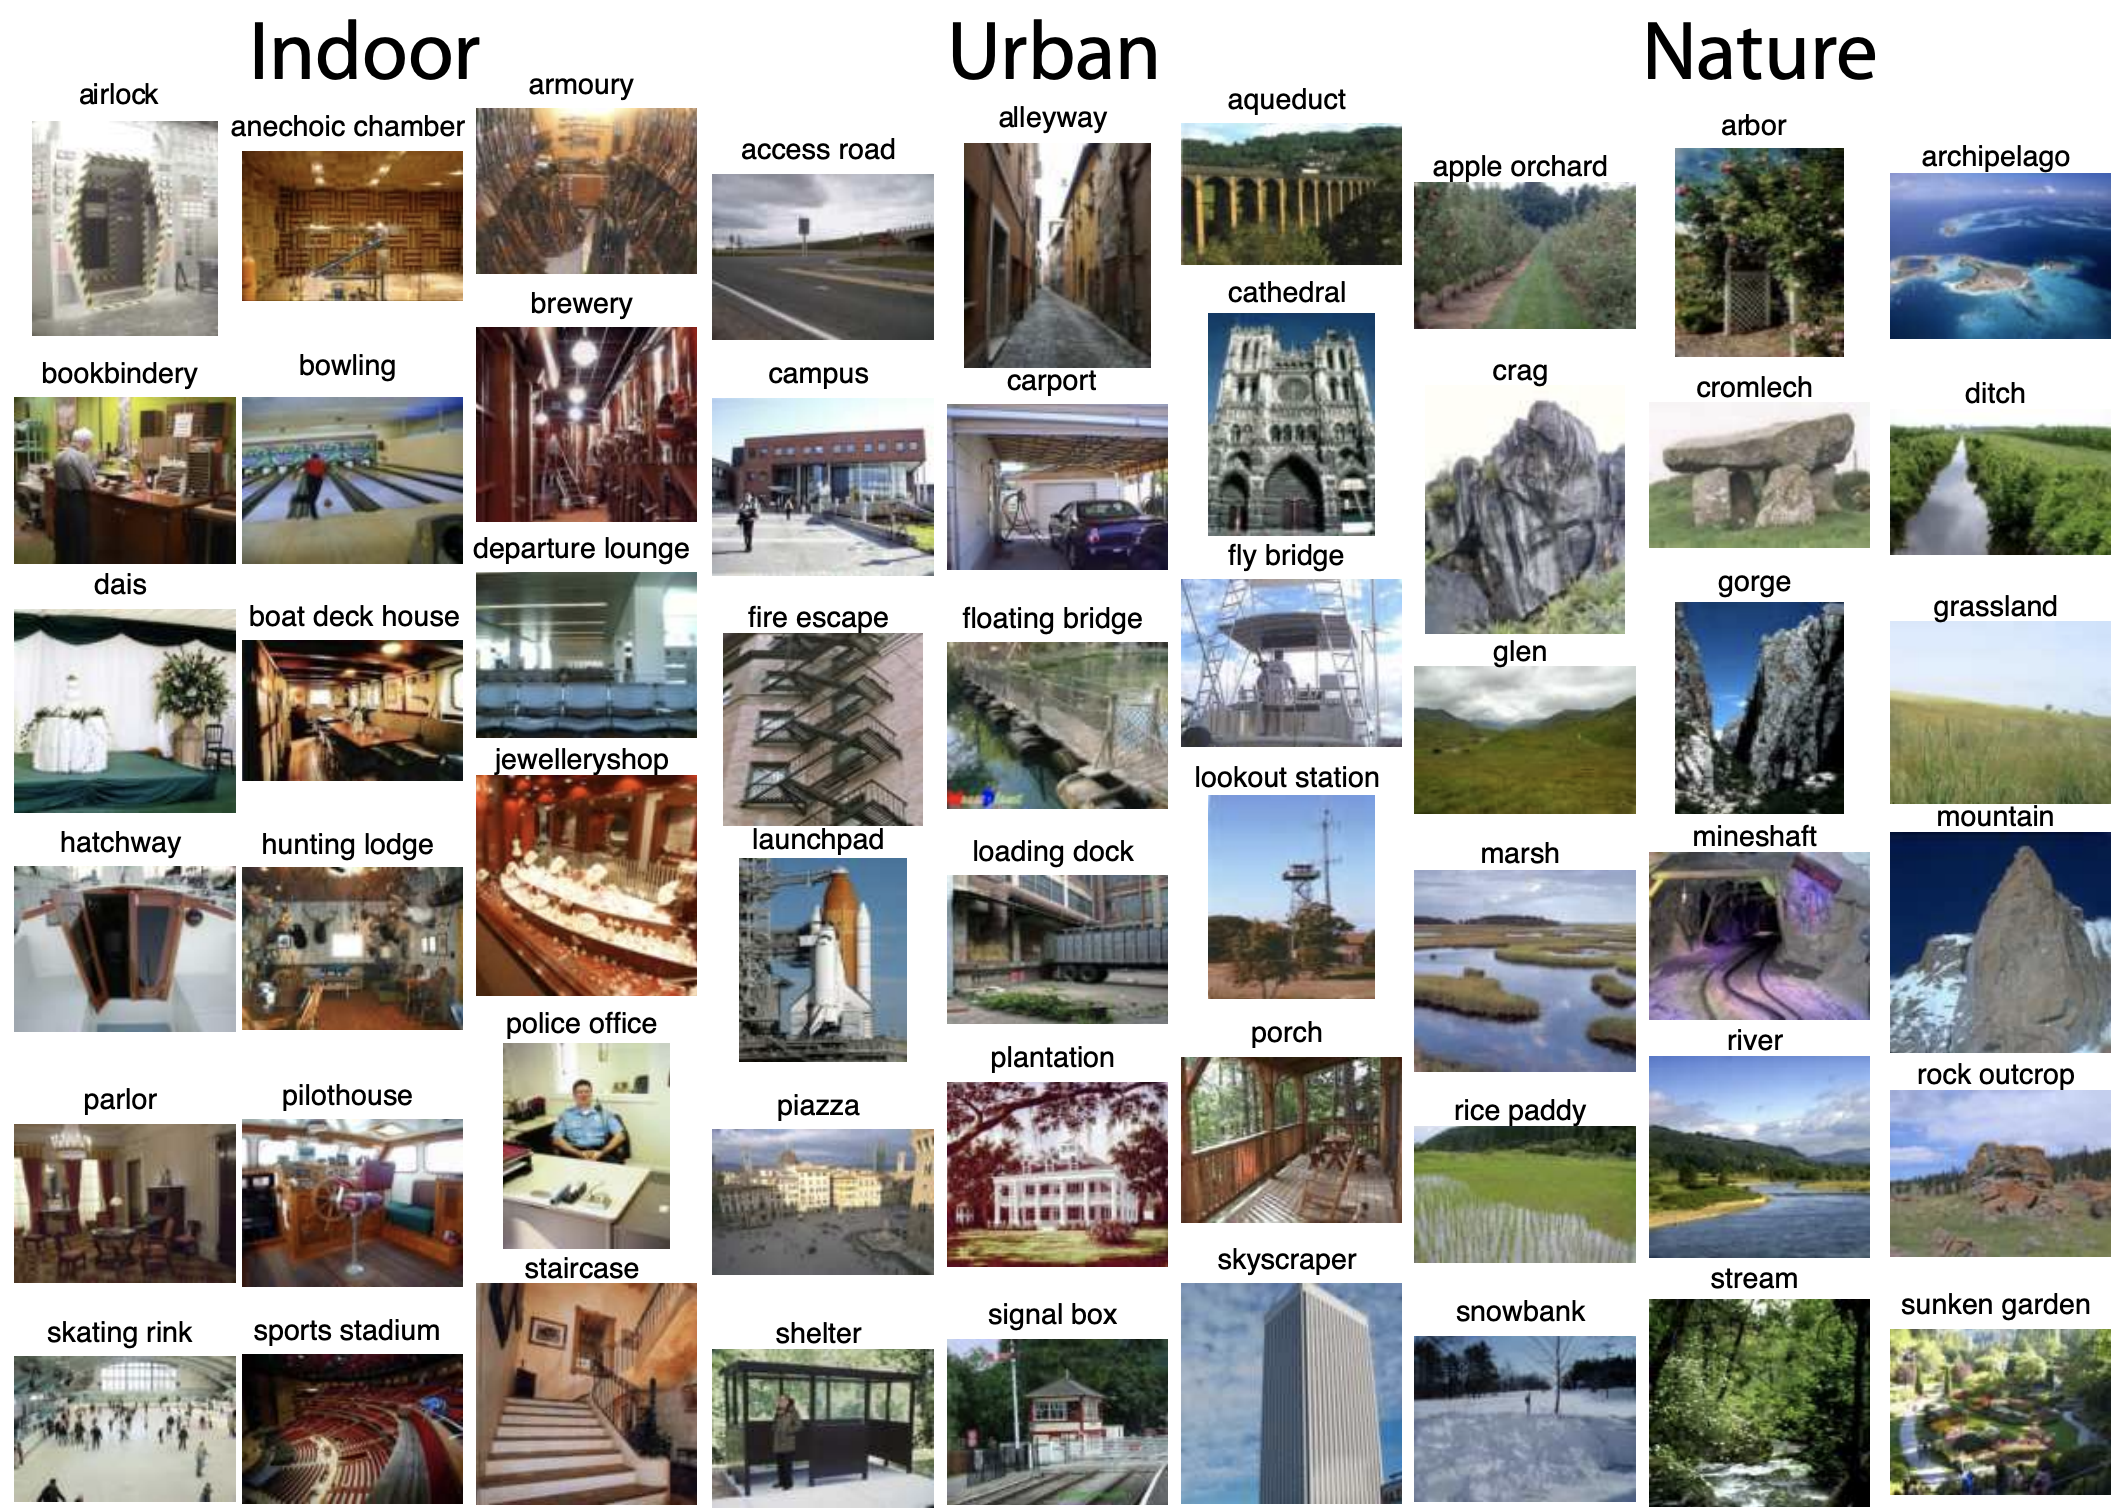
\includegraphics[width=0.95\linewidth]{Sun}
   	\end{center}
   	\caption{Примеры размеченных фотографий из датасета \textit{SUN}.}
   	\label{tikzpicture: sun}
\end{figure}

Ознакомиться с другими изображениями из датасета \textit{SUN} можно через 
интерактивный веб-обозреватель\footnote{groups.csail.mit.edu/vision/SUN/}, которым
можно воспользоваться для просмотра упорядоченных изображений как 
по сценам, так и по объектам.


\subsection{Адоптация датасета SUN}

\indent
\indent
Как было сказано в главе, посвященной постановке задачи,
 названия локаций (сцен) из датасета \textit{SUN} не 
являются сами по себе популярными тегами из социальных сетей. Поэтому 
прежде всего необходимо выполнить сопоставление. Условно можно
разбить процедуру сопоставления на 2 части: объединение исходных классов 
датасета \textit{SUN} в семантические домены и сопоставление полученных доменов
с популярными хэштегами. В качестве источника хэштегов была выбрана социальная
сеть \textit{Instagram}\footnote{www.instagram.com}, ориентированная на обмен фото
и видео контентом между пользователями.

\indent
Итак, предварительно необходимо очистить названия классов \textit{SUN} от служебных
слов и символов, таких как \textit{indoor, outdoor, exterier, interier}, знаков "/" и 
однобуквенных алфавитных указателей. Затем для полученных слов или 
словосочетаний подбирается соответствующий синсет из базы знаний \textit{Wordnet}.
Далее для синсетов находились гиперонимы, которые либо уже были достаточно
абстрактны, чтобы представлять собой часто встречающийся тег, либо 
автор работы находил для синсетов обобщающее понятие вручную.
Несколько примеров приведено в таблице~\ref{tabular: mapping}.


% Таблица о сопоставлении классов и тегов
\begin{table}[h]
    \begin{center}
        \begin{tabular}{c | c| c | c | c}
            \hline
            № & Исходное название & Синсет & Гипероним & Хэштег \\
            \hline
    
            1 & /s/shoe\_shop & shoe shop & shop & \htag{shopping} \\
    
            2 & /t/toyshop & toyshop & shop & \htag{shopping} \\
   
            3 & /v/volleyball\_court/indoor & volleyball court & court & \htag{sport} \\
    
            4 & /w/wrestling\_ring/indoor & wrestling ring & ring  & \htag{sport} \\
    
            5 & /r/rainforest & rain forest & forest & \htag{forest} \\
            
            6 & /p/pantry & pantry & storeroom & ? \\
   
            \hline
        \end{tabular}
    \end{center}
    \caption{Сопоставление искомых классов и хэштегов.}
    \label{tabular: mapping}
\end{table}


\indent
Из таблицы~\ref{tabular: mapping} видно, что некоторые синсеты имеют общие
гиперонимы. Кроме того, некоторые гиперонимы без каких-либо
дополнительных изменений могли быть использованы пользователями в качестве 
тегов. Таким образом, использование гиперонимов позволило немного уменьшить
количество ручной работы. Так же в таблице~\ref{tabular: mapping} приведен пример,
когда для локации сложно подобрать какой-то подходящий и широко распространенный
тег.  В итоге использовалось около половины из  \textit{397}
искомых классов датасета \textit{SUN}, каждому из которых удалось поставить
в соответствие один из \textit{20} популярных хэштегов. В данной работе 
популярными считаются теги, использованные в сети
\textit{Instagram} более \textit{10 млн.} раз. При этом среднее число упоминаний 
отобранных тегов составило \textit{100 млн.} раз, а
максимальное --- \textit{450 млн.}. Полная информация о встречаемости
хэштегов в сети \textit{Instagram} приведена на рисунке ~\ref{tikzpicture: tags_counts},
а о встречаемости в датасете \textit{SUN} -- на рисунке \ref{tikzpicture: sun_tags}.


% Гистограмма встречаемости хэштегов
\begin{center}
    \begin{figure}[h!]
    \begin{tikzpicture}
    \label{tags_counts}
        \begin{axis}[
            ylabel = Число упоминаний\, млн.,
            x tick label style={rotate=90,anchor=east},
            width = 0.7\paperwidth,
            height = 0.4\paperheight,
            symbolic x coords=
            {
                art,
                nature,
                sky,
                home,
                shopping,
                artchitecture,
                snow,
                water,
                sport,
                cars,
                street,
                cafe,
                garden,
                forest,
                bar,
                church,
                airport,
                window,
                entertainment,
                science
            },
            xtick=data
          ]
            \addplot[ybar,fill=blue] coordinates {
                (art, 450)
                (nature, 390)
                (sky, 190)
                (home, 115)
                (shopping, 100)
                (artchitecture, 97)
                (snow, 85)
                (water, 65)
                (sport, 60)
                (cars, 55)
                (street, 55)
                (cafe, 45)
                (garden, 41)
                (forest, 30)
                (bar, 25)
                (church, 25)
                (airport, 14)
                (window, 12)
                (entertainment, 11)
                (science, 10)
            };
        \end{axis}
    \end{tikzpicture}
    \caption{Встречаемость отобранных хэштегов в социальной сети \textit{Instagram}.}
    \label{tikzpicture: tags_counts}
    \end{figure}
\end{center}


\begin{figure}[h!]
    \begin{center}
   	    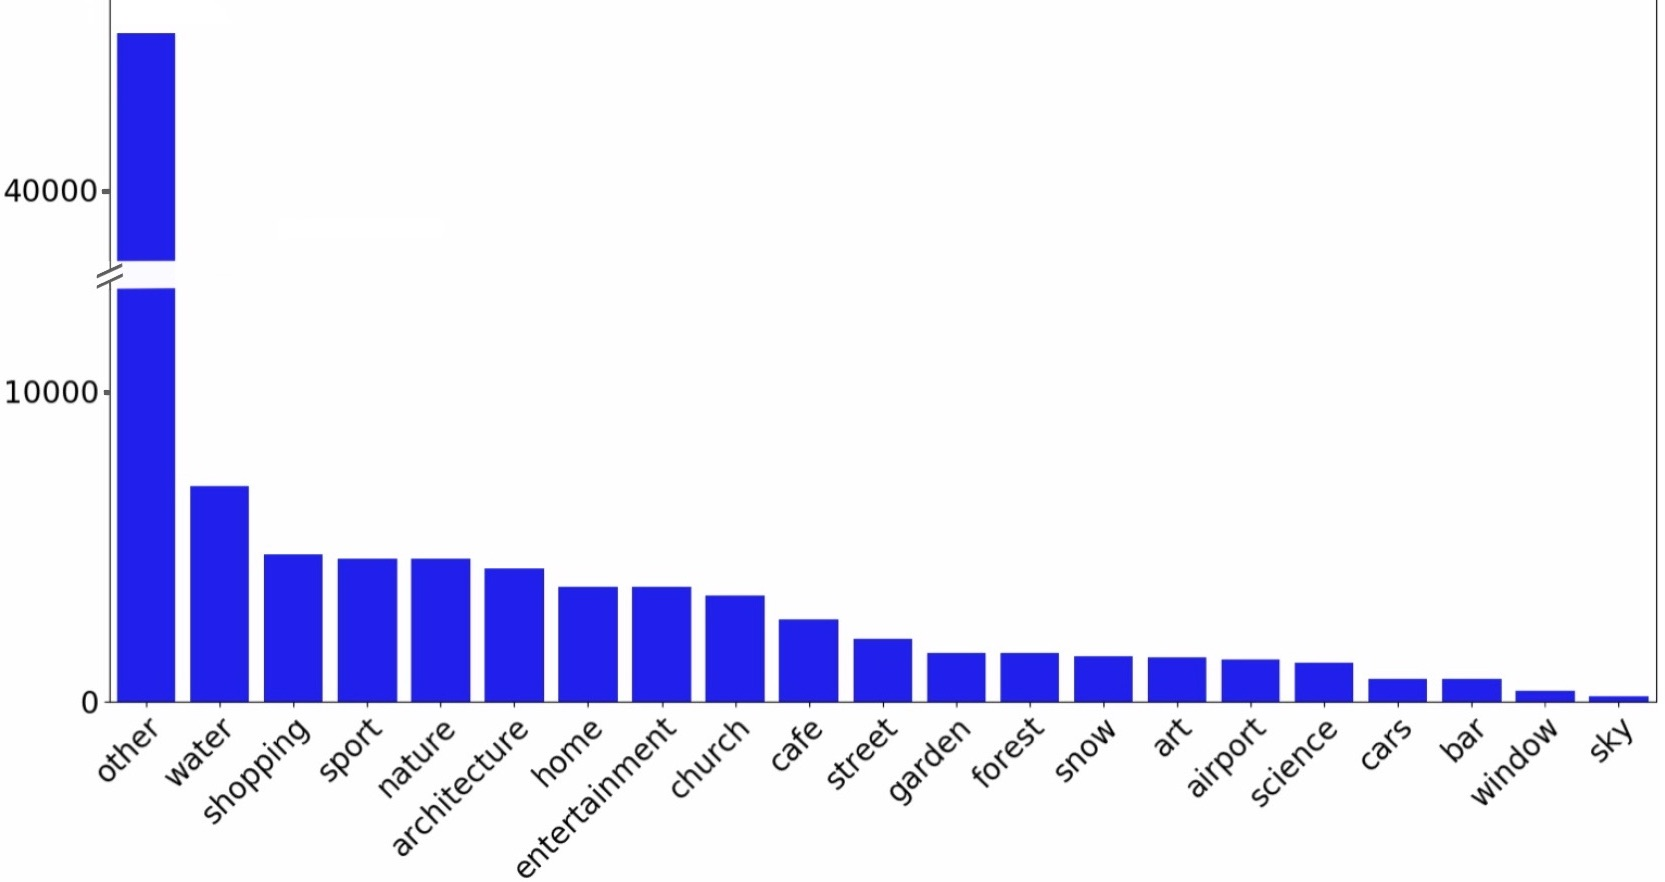
\includegraphics[width=0.95\linewidth]{sun_tags}
   	\end{center}
   	\caption{Распределение хэштегов в датасете \textit{SUN}.}
   	\label{tikzpicture: sun_tags}
\end{figure}



\indent 
Отметим, что автор предпринял несколько попыток произвести процедуру 
адаптации разметки датасета \textit{SUN} полностью автоматически, 
но они оказались неудачными. 


\indent
\indent
Первая попытка --- обобщить искомые классы, используя метод \textit{topic\_domains},
который доступен для синсетов в \textit{python} реализации API к 
базе \textit{WordNet}. Например, для синсета
\textit{basketball\_court.n.01}, который определяется как 
\textit{the court on which basketball is played}, 
вызов данного метода возвращает \textit{basketball.n.02}, который определяется так:
\textit{a game played on a court by two opposing teams of 5 players;
points are scored by throwing the ball through an elevated horizontal hoop}.
К сожалению, проблема заключалась в том, что для подавляющего числа названий 
локаций \textit{topic\_domains} возвращал пустое значение, т.е. для этих синсетов
авторами базы знаний не было назначено доменов.


\indent
\indent
Вторая попытка была аналогична первой, но использовалась сторонняя база знаний
\textit{WordNet Domains}\footnote{http://wndomains.fbk.eu/}. К сожалению, такое
расширение базы доменов не позволило решить проблему, описанную выше.


\indent
\indent
Третья идея заключалась в использовании информации о семантической близости 
синсетов, в частности, API \textit{WordNet'a} позволяет для любых двух синсетов
вычислить степень похожести несколькими способами:
\textit{jcn\_similarity, lch\_similarity, res\_similarity, wup\_similarity}.
Для разных видов измерения расстояния были вычислены матрицы попарных дистанций,
на основе которых производилась иерархическая кластеризация с различными
гиперпараметрами
 (например, кластеризация по заданному максимальному расстоянию в кластере, 
по заданному количеству кластеров). К сожалению, автору не удалось получить кластеры,
большую часть которых можно было бы без труда "озаглавить" 
каким-либо популярным хэштегом.


\indent
\indent
Таким образом, процедуру сопоставления всех 
\textit{397} искомых классов датасета \textit{SUN} и хэштегов из социальной сети \textit{Instagram}
пришлось произвести в полуручном режиме (опираясь только на гиперонимы),
как это было описано выше в данном разделе.


\indent
\indent
Приведем объединения исходных классов в домен. В таблице \ref{tabular: sport_classes} 
перечислены названия локаций, которым поставлен в соответствие хэштег \htag{sport}.

\begin{table}[ht!]
    \begin{center}
        \begin{tabular}{c | c | c}
            /w/wrestling\_ring/indoor &
            /a/athletic\_field/outdoor &
            /b/badminton\_court/indoor
            \\
            /b/ball\_pit &
            /b/baseball\_field &
            /b/basketball\_court/outdoor
            \\
            /b/boxing\_ring &
            /b/bullring &
            /g/golf\_course
            \\
            /g/gymnasium/indoor &
            /m/martial\_arts\_gym &
            /r/racecourse
            \\
            /r/riding\_arena &
            /s/ski\_lodge &
            /s/ski\_resort
            \\
            /s/ski\_slope &
            /s/squash\_court &
            /s/stadium/baseball
            \\
            /s/stadium/football &
            /s/swimming\_pool/indoor &
            /s/swimming\_pool/outdoor
            \\
            /t/tennis\_court/indoor &
            /t/tennis\_court/outdoor &
            /v/volleyball\_court/indoor
            \\
            /v/volleyball\_court/outdoor          
        \end{tabular}
    \end{center}
    \caption{Список классов датасета \textit{SUN}, которым сопоставлен хэштег \htag{sport}.}
    \label{tabular: sport_classes}
\end{table}

Файлы с полной информацией об итоговом сопоставлении искомых
классов и хэштегов можно найти в 
репозитории автора\footnote{github.com/AlekseySh/scenes}.